\chapter{Функционално програмиране}

\setcounter{section}{21}

\section {Уводни задачи}

\begin{enumerate}

  \item Да се дефинира функция, която намира лицето на триъгълник по дадени: а) дължини на страна и височина към нея; б) три страни.
  
  \item Да се дефинира функция, която по двойка $(x,y)$ коррдинати на точка от равнината намира на кой квадрант принадлежи точката. Да се разгледат случаите, когато точката принадлежи на някоя от координатните оси или съвпада с центъра на координатната система.

  \item Да се дефинира функция, която  има стойност истина, ако посоченото условие е вярно и стойност - лъжа, в противен случай:

	\renewcommand{\theenumii}{\Alph{enumii}}

	\begin{enumerate}[label=\alph*)]%[a)] % a), b), c), ...
			 \item цялото число p се дели на 4 или на 7;
			 \item уравнението $ax^2 + bx + c = 0 (a \neq 0)$ няма реални корени;
			 \item точка с координати (a, b) лежи във вътрешността на кръг с радиус 5 и център (0, 1); г) точка с координати (a, b) лежи извън кръга с център (c, d) и радиус f;
			 \item точка принадлежи на частта от кръга с център (0, 0) и радиус 5 в трети квадрант;
			 \item точка принадлежи на венеца с център (0, 0) и радиуси 5 и 10;
			 \item x принадлежи на отсечката [0, 1];
			 \item x е равно на max \{a, b, c\};
			 \item x е различно от max \{ a, b, c\};
			 \item нито едно от числата a, b и c не е положително;
			 \item цифрата 7 влиза в записа на положителното трицифрено число p;
			 \item цифрите на трицифреното число m са различни;
			 \item поне две от цифрите на трицифреното число m са равни помежду си;
			 \item цифрите на трицифреното естествено число x образуват строго растяща или строго намаляваща редица;
			 \item десетичните записи на трицифрените естествени числа x и y са симетрични;
			 \item естественото число x, за което се знае, че е по-малко от 23, е просто.
  \end{enumerate}

  \item Да се напише функция, която намира броя на цифрите в десетичния запис на дадено естествено число.
  
  \item Да се напише функция, която намира сумата на цифрите в десетичния запис на дадено естествено число.
  
  \item Да се дефинира функцията $pow(x,k)=x^k$ за цели положителни числа $x$ и $k$.
  
  \item Да се напише функция, която по дадени естествено число $x$ и едноцифрено числа $k$ намира а)дали $k$ се среща в десетичния запис на $x$ и б) колко пъти $k$ се среща в десетичния запис на $x$.
  
  \item Да се напише функция, която проверява дали дадена година е високосна. (вж. задача 2.12. в \cite{sbornik})
  
  \item Да се напише функция, която по дадено естествено число n ($n \geq 1$) намира броя на тези елементи от серията числа $i^3 + 13 \times i \times n + n^3$ , $i = 1, 2, ..., n$, които са кратни на 5 или на 9.

  \item Да се дефифира функция, която по естествени числа $n$ и $k$ намира дали $n$ е точна степен на числото $k$.

  \textit{Упътване: Разделете променливата $n$ на променливата $k$ ``колкото пъти е възможно'' и проверете дали $n$ достига единица или някое друго число след края на процеса. Използвайте оператора за намиране на остатък при целочислено деление и оператора за целочислено деление.}

  \item Едно положително цяло число е съвършено, ако е равно на сумата от своите делители (без самото число). Например, 6 е съвършено, защото 6 = 1+2+3; числото 1 не е съвършено. Да се дефинира функция, която проверява дали дадено положително цяло число е съвършено.


  \section {Конструиране на списъци}

  \item Да се съставят следните списъци:
	\renewcommand{\theenumii}{\Alph{enumii}}

	\begin{enumerate}[label=\alph*)]%[a)] % a), b), c), ...
			 \item Първите $n$ четни числа;
			 \item Първите $n$ члена на аритметична прогресия с първи член $a$ и разлика $d$;
			 \item $[1!, 2!, ..., n!]$ за дадено $n$;
			 \item Всички четни числа;
			 \item Всички членове на аритметична прогресия с първи член $a$ и разлика $d$;
			 \item $[1!, 2!, ...]$ (безкраен списък)
  \end{enumerate}

  \item Да се дефинира функция, която по дадено естествено число $n$ връща списък с цифрите му, четени отдясно на ляво.

  \item(*) Да се дефинира функция, която по дадено естествено число $n$ връща списък с цифрите му, четени отдясно на ляво, без повторения на елементите на списъка.

  \item Едно положително цяло число е съвършено, ако е равно на сумата от своите делители (без самото число). Например, 6 е съвършено, защото 6 = 1+2+3; числото 1 не е съвършено. Да се дефинира функция, която създава списък с  всички съвършени числа, ненадминаващи дадено положително цяло число в параметър $n$.
  
  \item Да се дефинира функция $histogram$, която по символен низ $s$ връща списък от двойки $(c_i,n_i)$, където $c_i$ са различните символи от $s$, а $n_i$ е броя на срещания на $c_i$ в $s$. Например, $histogram \: "abracadabra" \rightarrow [(a,5), (b,2), (r,2), (c,1), (d,1)]$. Използвайте помощни функции.
\end{enumerate}

\section {Работа със списъци и образци}

\begin{enumerate}[resume]

	\item Дефинирайте функция $say$, която по едноцифрено цяло число връща неговото наменование. Например, $say \: 3 \rightarrow "three"$.

	\item Да се дефинира функция, която по два списъка намира дължината на най-дългия им общ префикс.

	\item Да се дефинира функция $countEvenOdd \: l$, която за списъка от цели числа $l$ връща наредена двойка от броя на четните и броя на нечетните числа в $l$.

	\item Да се дефинира функция $pivot \: l \: x$, която за списъца от числа $l$ и числото x връща наредена двойка $(l_1,l_2)$, където $l_1$ е списък от елементите на $l$, по-малки от $x$, а $l_2$ е списък от елементите на $l$, по-големи или равни на $x$.
	
	\item Да се дефинира функция, която в даден низ замества всички малки латински букви със съответните им големи латински букви.
	
	\item Да се дефинира функция, която проверява дали даден низ е палиндром, т.е. дали се е еднакъв при четене от ляво на дясно и от дясно на ляво.
	
	\item Да се дефинира функция, която по даден списък от цели числа $l$ връща списък от всички двойки $(a,b)$ от $l$, за които $a$ и $b$ са съседни елементи в $l$ и $a < b$.
	
	\item Да се дефинира функция \code{groupsof l x}, която разделя списъка $l$ на групи от по $x$ елемента. 
	
	Например, $groupsof \: [1,2,3,4,5,6,7,8] \: 3 \rightarrow [[1,2,3],[4,5,6],[7,8]]$.

	\item Да се дефинира функция $flatten \: \: l :: [[a]] \rightarrow [a]$, която получава списък от списъци и връща списък, който съдържа всички елементи на входните списъци.

	\item Да се дефинира функция $decode \: l :: [(Int,a)] \rightarrow [a]$, която получава списък от двойки и връща списък, който съдържа всички елементи на входния списък, като всеки елемент се повтаря толкова пъти, колкото е указано в първия елемент на двойката.

	\item Да се дефинира функция $pack \: l :: [a] \rightarrow [[a]]$, която получава списък и връща списък от списъци, като всеки от тях съдържа всички последователни еднакви елементи на входния списък.
	
	Например, $pack \: [1,1,1,2,2,3,4,4,4,4] \rightarrow [[1,1,1],[2,2],[3],[4,4,4,4]]$.

	\item Да се дефинира функция $encode \: l :: [a] \rightarrow [(Int,a)]$, която получава списък и връща списък от двойки, където първият елемент на двойката е броят на последователните еднакви елементи от входния списък, а вторият елемент е самият елемент.
	
	Например, $encode \: [1,1,1,2,2,3,4,4,4,4] \rightarrow [(3,1),(2,2),(1,3),(4,4)]$.

	\item Да се дефинира функция \code{remove x l}, която премахва (а) първото срещане на елемента $x$ от списъка $l$ и (б) всички срещания на елемента $x$ от списъка $l$.
		
	\item Да се дефинира функция \code{removeDuplicates l}, която премахва всички повторения на елементите на списъка $l$.
	
		

\end{enumerate}



\section {map, filter, fold}

\begin{enumerate}[resume]
	\item Направете и тествайте собствена реализация на функциите \code{map}, \code{filter} и \code{fold(l,r,l1,r1)}.
	\item Нека е даден списък \code{l::[(Int,Int,Int)]} с тройки $(a_i,b_i,c_i)$. С помощта на \code{map}, \code{fold} и \code{filter} да се намерят:
	
	\begin{enumerate}[label=\alph*)]
		\item Списъка от сумите на елементите на тройките $[(a_i+b_i+c_i)]$
		\item Тройка от сумите на отделните компоненти на елемнтите на \code{l}, $(\sum a_i,\sum b_i, \sum c_i)$
		\item Броя на тройките, за които $a_i+b_i>c_i$
		\item Дали има поне една тройка, за която $a_i=b_i=c_i$ (\code{True} или \code{False})
	\end{enumerate}
\end{enumerate}


\begin{mdframed}[hidealllines=true,backgroundcolor=gray!20]
На лекции разглеждаме модел на лабиринт, сържащ цел и препятсвия.
\begin{lstlisting}[basicstyle=\small,language=Haskell]
type Pos = (Int, Int)
  
data Tile = Road | Wall | Gold
            deriving (Show, Eq)  
data Game = Game { pos :: Pos, world :: [[Tile]]}
            deriving (Show)
myWorld :: Game = Game { pos = (0, 0), 
                         world = [[Road, Wall, Gold], 
                                  [Road, Wall, Road], 
                                  [Road, Road, Road]]}
\end{lstlisting}
\begin{center}
	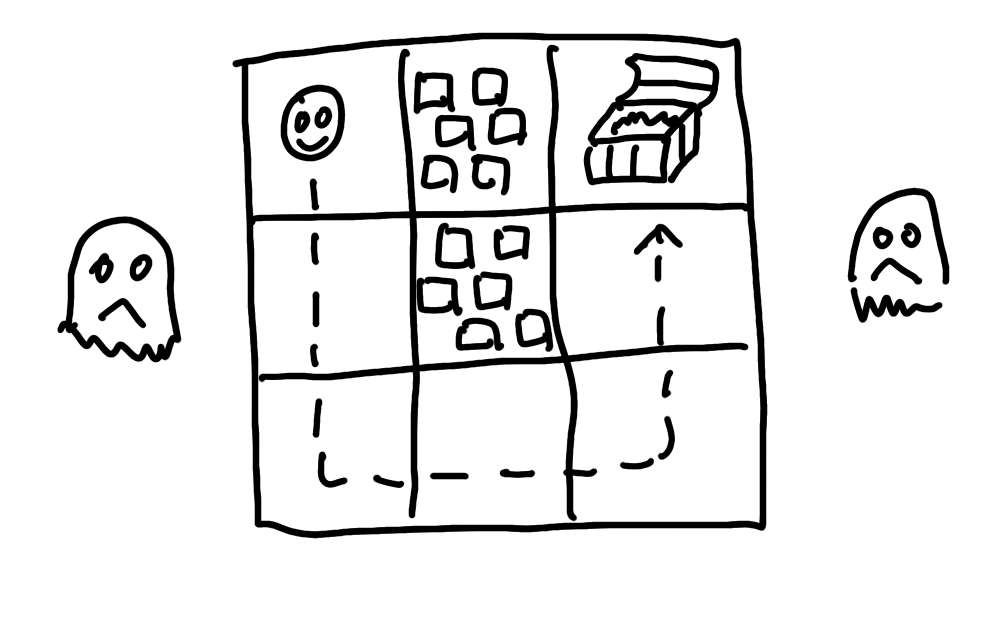
\includegraphics[width=4cm]{images/maze}	
\end{center}

Следите функции ``придвижват'' играча в лабиринта:

\begin{lstlisting}[basicstyle=\small,language=Haskell]
left (Game (x, y) w) = Game (x-1, y) w
right (Game (x, y) w) = Game (x+1, y) w
up (Game (x, y) w) = Game (x, y-1) w
down (Game (x, y) w) = Game (x, y+1) w	
\end{lstlisting}

И помощни функции при изследване на играта:

\begin{lstlisting}[basicstyle=\small,language=Haskell]
foundGold  :: Game -> Bool
foundGold  (Game (x,y) w) = (w !! y) !! x == Gold
stuck  :: Game -> Bool
stuck  (Game (x,y) w) = dead w (x, y)
dead :: [[Tile]] -> Pos -> Bool
dead w (x, y) = x < 0 || x >= length w ||
                y < 0 || y >= length w || 
                (w !! y) !! x == Wall
move :: Game -> (Pos -> Pos) -> Maybe Game
move (Game p w) mv = if dead w (mv p) 
                       then Nothing 
                       else Just $ Game (mv p) w
\end{lstlisting}

\end{mdframed}

\begin{enumerate}[resume]
	\item С помощта на \code{map}, \code{mapMaybe}, \code{filter} и \code{fold} да се намерят:
	\begin{enumerate}[label=\alph*)]
		\item Броя на препятсвията в даден лабиринт
		\item Броя съседи на целта, които не са препятсвия
		\item Дали целта е оградена изцяло от препятствия (\code{True} или \code{False})
	\end{enumerate}

	\item(*) С помощта на \code{foldr} да се дефинира функция, която проверява дали дали даден списък от числа \code{l::[Int]} е нареден във възходящ ред. \emph{Упътване: Използвайте двойка \code{(Bool,Int)} за акумулатор.}

\end{enumerate}